\chapter{Реализация ключевых решений}
\label{cha:impl}

\section{OpenAPI-генерация кода}

Одним из ключевых достижений является полная генерация серверного кода по OpenAPI-спецификации~\cite{oapi:codegen}. Инструмент \Code{oapi-codegen} принимает файл \Code{openapi/openapi.yaml} и создаёт типы данных, интерфейс StrictServerHandler и HTTP-маршрутизатор.

Разработчику достаточно реализовать методы заданного интерфейса. Аналогично для десктопного клиента: OpenAPI Generator (cpp-qt-client)~\cite{openapi:generator} из той же спецификации генерирует класс \Code{OAIDefaultApi} со всеми методами API.

Таким образом обеспечивается консистентность API-моделей между клиентской и серверной частями приложения. В связи с этим сгенерированный код рассматривается исключительно как производный результат и не предполагает ручного редактирования: все изменения должны вноситься на уровне OpenAPI-спецификации с последующей повторной генерацией кода.

\section{Импорт расписания из XLSX}

Модуль импорта реализован в пакете \Code{internal/lib/xlsxParser.go}. Класс \Code{Parser} выполняет разбор XLSX-файлов в формате, используемом диспетчерской службой ПНИПУ.

Основные этапы работы:
\begin{enumerate}
\item разархивация ZIP-файла, полученного через multipart-форму из функции вызывающего хендлера;
\item построчный обход XLSX-таблицы для каждой учебной группы;
\item парсинг ячейки занятия с помощью регулярных выражений;
\item формирование staging-данных и возврат их в хендлер;
\item вставка данных во временные таблицы;
\item сравнение хешей для избежания дублирования;
\item перенос в основные таблицы.
\end{enumerate}

\section{Экспорт в iCalendar}

Модуль экспорта реализован в пакете \Code{internal/lib/icsSerializer.go}. Функция \Code{SerializeICS} принимает список занятий и возвращает байтовый массив в формате iCalendar. Экспорт доступен через REST API и в том числе реализован в десктопном клиенте.

\section{Десктопный клиент на Qt6}

Десктопный клиент использует сгенерированный по OpenAPI-спецификации класс \Code{OAIDefaultApi}. Все сетевые вызовы асинхронны (сигналы Qt), что обеспечивает отзывчивость интерфейса. Каждый редактор сущности содержит поля для отображения и изменения данных, кнопки сохранения и удаления, подключаемые к соответствующим сигналам API.

Визуализация расписания реализована через \Code{TimetablePainter}, отрисовывающий недельную сетку: дни недели по горизонтали, временная линейка по вертикали, занятия в виде цветных блоков.

Каждый виджет занятия отображает время проведения, наименование дисциплины, а также поддерживает отображение нескольких преподавателей и учебных групп. Цвет блока соответствует типу занятия: лекция, практика, КСР, лабораторное занятие. Цвета взяты из официального бренд-бука Пермского национального исследовательского политехнического университета. Стили оформления приложения (шрифты, отступы, цветовая схема) заимствованы с официального сайта вуза pstu.ru, что обеспечивает визуальное единство с корпоративным стилем университета.

На рисунках~\ref{fig:mainwindow}--\ref{fig:pagination} представлены скриншоты ключевых экранов десктопного клиента.

\begin{figure}[H]
  \centering
  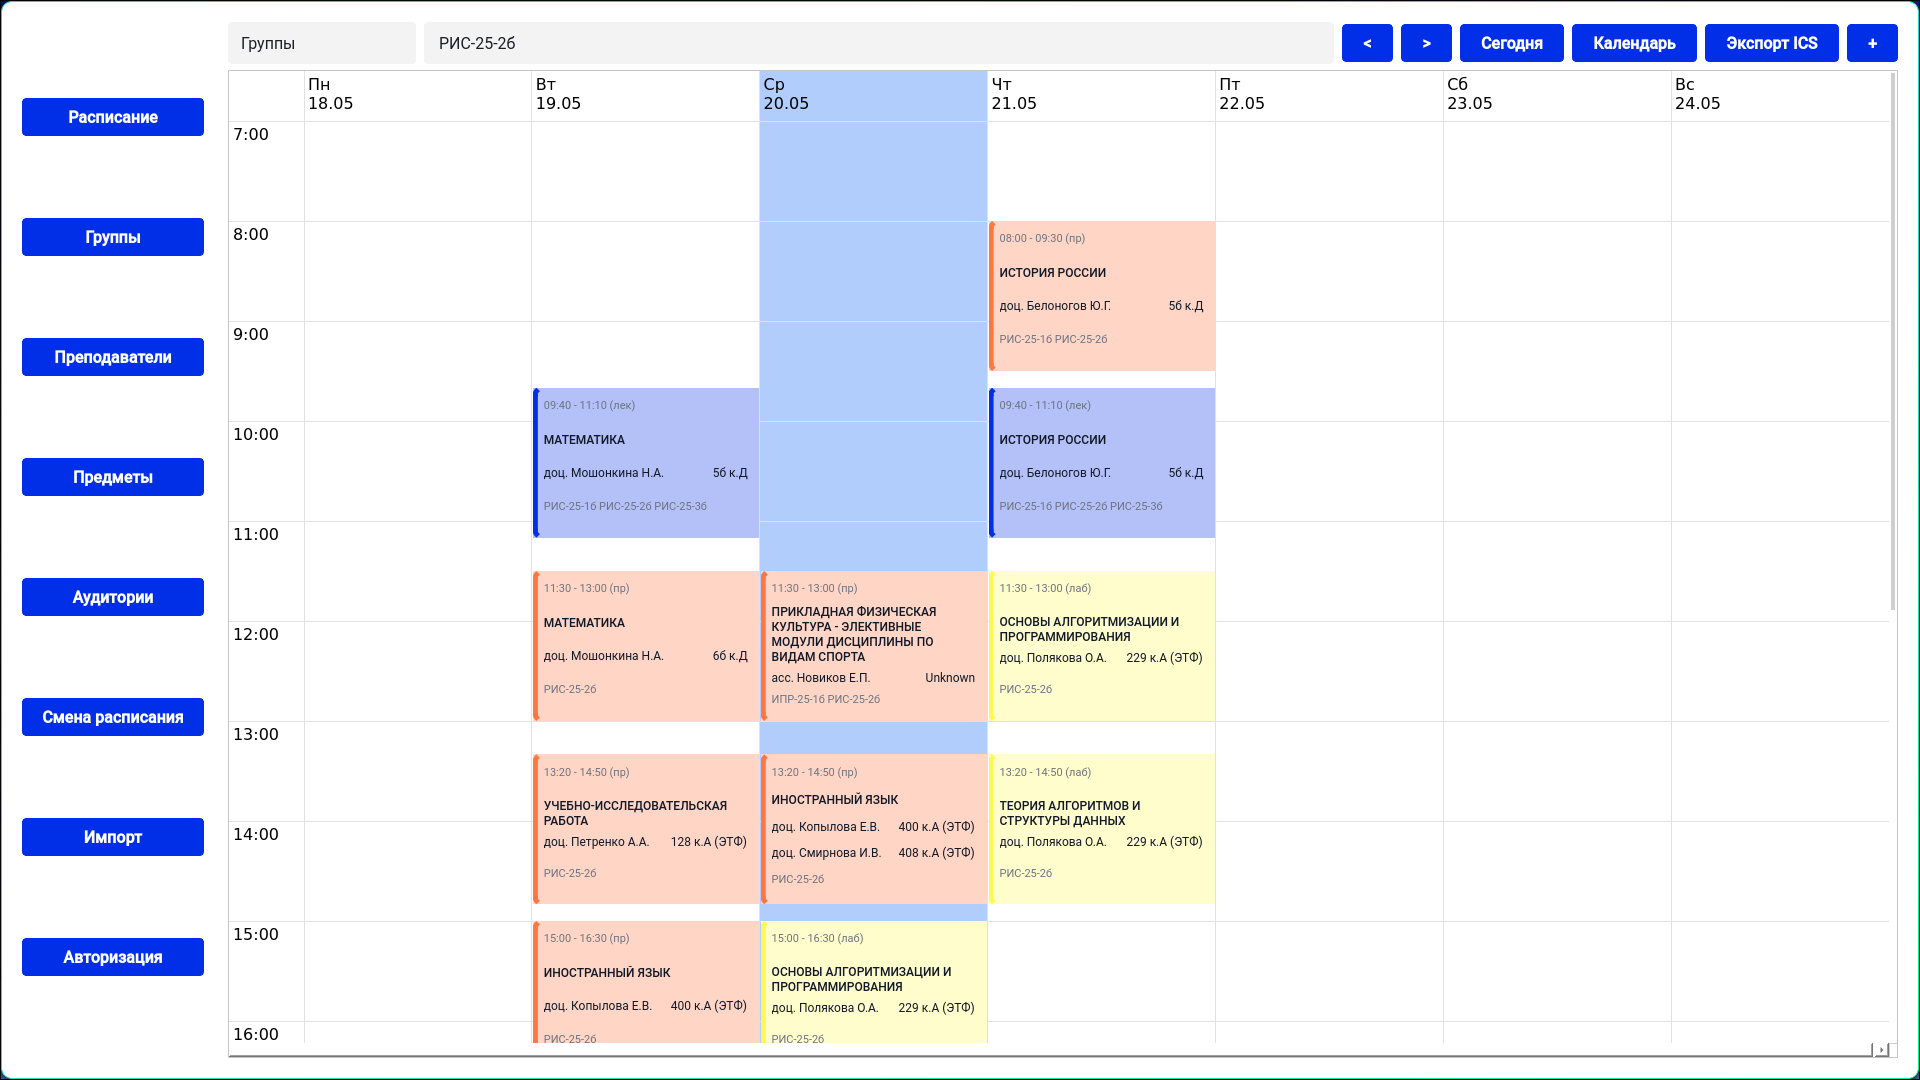
\includegraphics[width=\textwidth]{screenshot-timetable.png}
  \caption{Главное окно с недельной сеткой расписания}
  \label{fig:mainwindow}
\end{figure}

\begin{figure}[H]
  \centering
  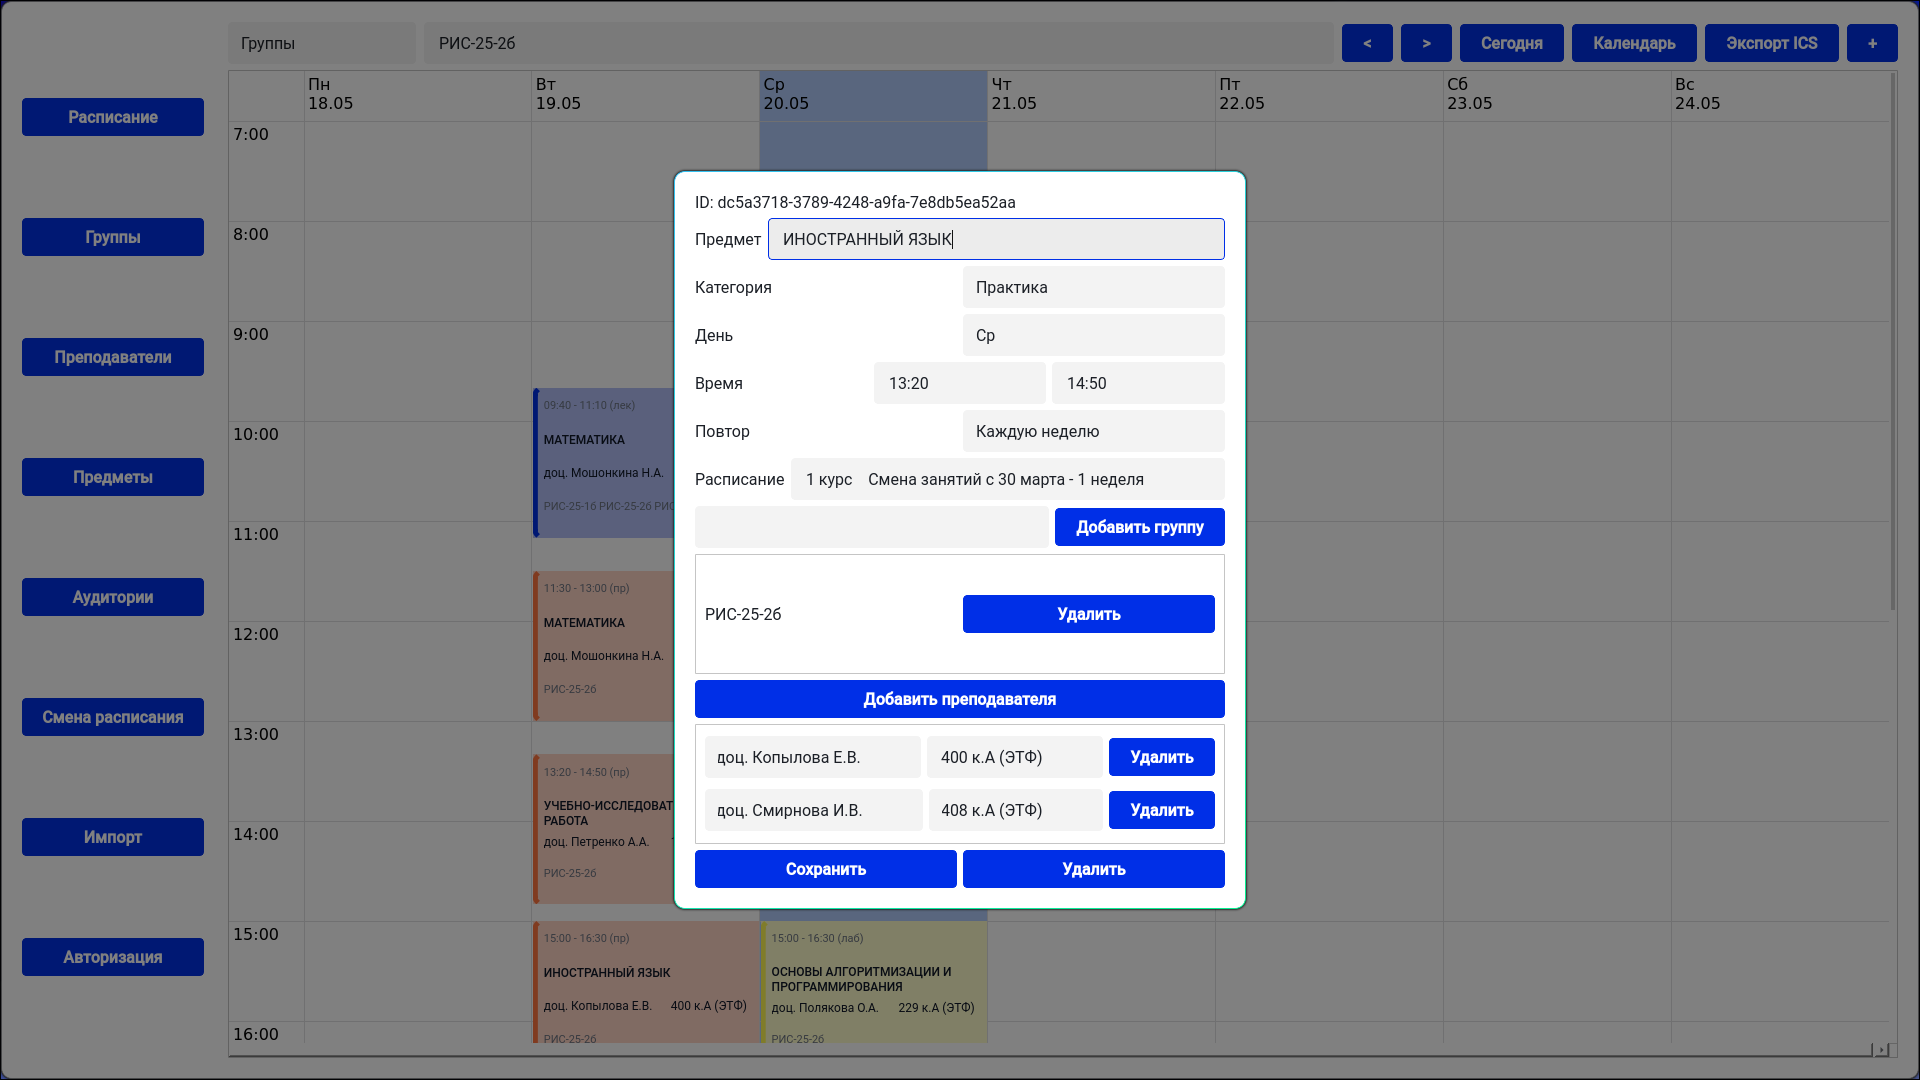
\includegraphics[width=\textwidth]{screenshot-lesson.png}
  \caption{Редактор занятия с привязкой преподавателя, аудитории и подгрупп}
  \label{fig:lesson}
\end{figure}

\begin{figure}[H]
  \centering
  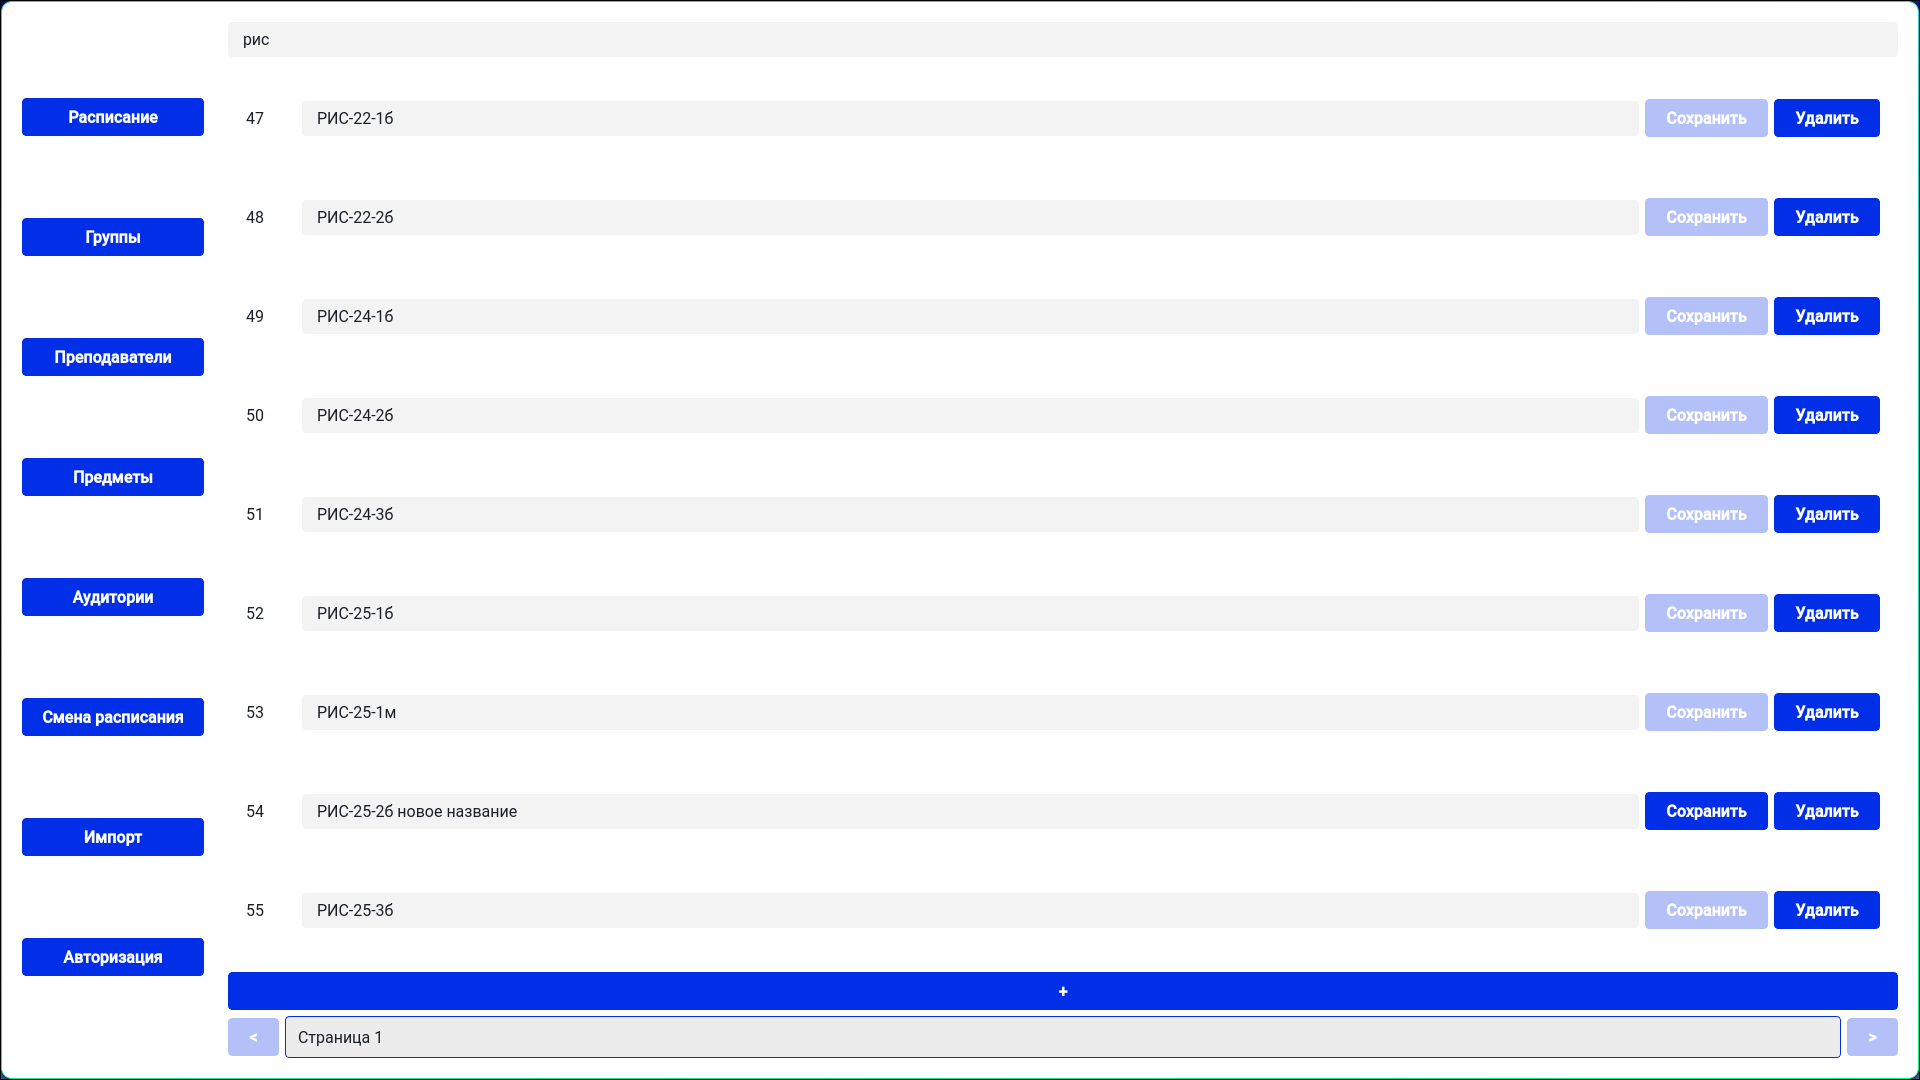
\includegraphics[width=\textwidth]{screenshot-list.png}
  \caption{Постраничный список сущностей с поиском}
  \label{fig:pagination}
\end{figure}

\section{Докеризация приложения}

Приложение полностью контейнеризировано. Docker Compose описает четыре сервиса:
\begin{itemize}
\item \textbf{postgres}---база данных PostgreSQL~16~\cite{postgres:doc};
\item \textbf{backend}---Go-сервер;
\item \textbf{frontend}---веб-интерфейс (React);
\item \textbf{nginx}---обратный прокси.
\end{itemize}

Запуск осуществляется одной командой \Code{docker compose up}.

\chapter{Результаты разработки}
\label{cha:results}

В результате работы разработано полнофункциональное клиент-серверное приложение. Приложение предоставляет диспетчеру следующие возможности:

\begin{itemize}
\item CRUD-управление справочными данными (группы, преподаватели, аудитории, дисциплины, семестры);
\item CRUD-управление занятиями с гибкой привязкой преподавателей и аудиторий;
\item импорт расписания из ZIP-архивов с XLSX-файлами формата ПНИПУ;
\item экспорт расписания в iCalendar сервисов календарей;
\item просмотр расписания в недельной сетке в десктопном приложении;
\item разграничение доступа по ролям.
\end{itemize}

Автор считает наиболее значимыми достижениями работы следующие:
\begin{enumerate}
\item \textbf{Импорт данных из Excel-файлов}---главное достоинство программы. Обеспечена совместимость с форматом файлов, используемым в ВУЗе. Программа автоматически обрабатывает время, дни недели, подгруппы (в том числе не заданные явно), чётность недели и прочие данные.
\item \textbf{OpenAPI-генерация кода}---единая спецификация автоматически генерирует сервер на Go и клиент на C++/Qt, исключая рассинхронизацию между API и клиентами.
\item \textbf{Экспорт iCalendar}---после однократной подписки студенту не требуется выполнять дополнительные действия: изменения, вносимые диспетчером, автоматически синхронизируются с календарём пользователя.
\item \textbf{Докеризация}---вся серверная часть запускается одной командой \Code{docker compose up}.
\end{enumerate}